\documentclass{article}
\usepackage{ctex}
\usepackage{graphicx}
\usepackage{ctex}
\usepackage{amsmath}
\usepackage{amsfonts}
\usepackage{amssymb}
\usepackage{enumerate}
\usepackage{color}
\usepackage{setspace}
\usepackage{pythonhighlight}
\usepackage{bm}

\usepackage
[a4paper,
text={146.4true mm,239.2 true mm},
top= 26.2true mm,
left=31.8 true mm,
head=6true mm,
headsep=6.5true mm,
foot=16.5true mm]
{geometry} % 设置文本的边距
\input{../setup/format}

\begin{document}
    \title{Homework 6 of Stochastic Processes}
    \author{姓名:林奇峰\qquad 学号:19110977}
    \maketitle

    \section{Exercise 4.8}
    A transition probability matrix [P] is said to be doubly stochastic if 
    \begin{equation*}
        \sum_j P_{ij}=1\quad\text{for all }i ,\quad\sum_i P_{ij}=1\quad\text{for all j.}
    \end{equation*}
    \

    That is, the row sum and the column sum each equal 1. If a doubly stochastic chain has $\text{M}$ states and is ergodic (i.e., has a single class of states and aperiodic), calculate its steady-state probabilities.

    \textbf{Solutions:}
    
    Since every Markov chain with $\text{M}<\infty$ states contains at least one recurrent set of states and the doubly stochastic chain has a single class of states and aperiodic, it means that the doubly stochastic chain is an ergodic unichain.

    For an ergodic unichain, there is unique steady-state vector $\bm{\pi}$ that is a left eigenvector with $\lambda=1$ and (within a scale factor) a unique right eigenvector $\bm{e}=(1,\dots,1)^{\text{T}}$.

    We can see that $\bm{e}^\text{T}[P]=1\cdot\bm{e}^\text{T}$, and thus by scaling $\bm{e}^\text{T}$ we can obtain the unique steady-state vector $\bm{\pi}$.

    Finally, $\bm{\pi}=\frac{1}{\text{M}}\bm{e}^\text{T}$.

    \section{Exercise 4.10}
    \begin{figure}[h]
        \centering
        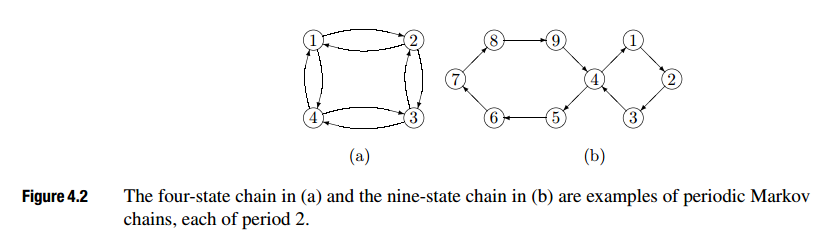
\includegraphics[width=5.5in]{figure_4_2.png}
    \end{figure}
    \begin{enumerate}[(a)]
        \item Find the steady-state probabilities for each of the Markov chains in Figure 4.2. Assume that all clockwise probabilities in the first graph are the same, say $p$, and assume that $P_{4,5}=P_{4,1}$ in the second graph.
        \item Find the matrices $[P^2]$ for the same chains. Draw the graphs for the Markov chains represented by $[P^2]$, i.e., the graph of two step transitions for the original chains. Find the steady-state probabilities for these two-step chains. Explain why your steady-state probabilities are not unique.
        \item Find $\lim_{n\rightarrow\infty}[P^{2n}]$ for each of the chains.
    \end{enumerate}
    \textbf{Solutions:}
    \begin{enumerate}[(a)]
        \item Solve the equation $\bm{\pi]}[P]=\bm{\pi}$directly with $\sum_i\pi_i=1$.
            
        For the first graph:
            \begin{equation*}
                \begin{aligned}
                    \bm{\pi}[P]&=\bm{\pi}\\
                    &\Downarrow\\
                    \bm{\pi}(I-[P])&=\bm{0}\\
                    &\Downarrow\\
                    \bm{\pi}\begin{bmatrix}
                        1 & -\frac{1}{2} & 0 & -\frac{1}{2}\\
                        -\frac{1}{2} & 1 & -\frac{1}{2} & 0\\
                        0 & -\frac{1}{2} & 1 & -\frac{1}{2}\\
                        -\frac{1}{2} & 0 & -\frac{1}{2} & 1\\
                    \end{bmatrix}
                    &=\bm{0}\\
                    &\Downarrow\\
                    \bm{\pi}&=(\frac{1}{4},\frac{1}{4},\frac{1}{4},\frac{1}{4})
                \end{aligned}
            \end{equation*}

        For the second graph:
            \begin{equation*}
                \begin{aligned}
                    \bm{\pi}\begin{bmatrix}
                        1 & -1 & 0 & 0 & 0 & 0 & 0 & 0 & 0\\
                        0 & 1 & -1 & 0 & 0 & 0 & 0 & 0 &0\\
                        0 & 0 & 1 & -1 & 0 & 0 & 0 & 0 &0\\
                        -0.5 & 0 & 1 & 0 & -0.5 & 0 & 0 & 0 &0\\
                        0 & 0 & 0 & 0 & 1 & -1 & 0 & 0 & 0\\
                        0 & 0 & 0 & 0 & 0 & 1 & -1 & 0 & 0\\
                        0 & 0 & 0 & 0 & 0 & 0 & 1 & -1 &0\\
                        0 & 0 & 0 & 0 & 0 & 0 & 0 & 1 &-1\\
                        0 & 0 & 0 & -1 & 0 & 0 & 0 & 0 &1\\
                    \end{bmatrix}&=\bm{0}\\
                    &\Downarrow\\
                    \bm{\pi}=(\frac{1}{10}, \frac{1}{10}, \frac{1}{10}, \frac{1}{5}, \frac{1}{10}, \frac{1}{10}, \frac{1}{10}, \frac{1}{10}, \frac{1}{10}, \frac{1}{10})
                \end{aligned}
            \end{equation*}

        \item For the first graph:
            \begin{equation*}
                [P^2]=\begin{bmatrix}
                    0.5 & 0    & 0.5  & 0\\
                    0   & 0.5  & 0    & 0.5\\
                    0.5 & 0    & 0.5  & 0\\
                    0   & 0.5  & 0    & 0.5\\
                \end{bmatrix}
            \end{equation*}


            For the second graph:
            \begin{equation*}
                [P^2]=\begin{bmatrix}
                0         & 0         & 1         & 0         & 0         & 0         & 0         & 0         & 0\\
                0         & 0         & 0         & 1         & 0         & 0         & 0         & 0         & 0\\
                0.5       & 0         & 0         & 0         & 0.5       & 0         & 0         & 0         & 0\\
                0         & 0.5       & 0         & 0         & 0         & 0.5       & 0         & 0         & 0\\
                0         & 0         & 0         & 0         & 0         & 0         & 1         & 0         & 0\\
                0         & 0         & 0         & 0         & 0         & 0         & 0         & 1         & 0\\
                0         & 0         & 0         & 0         & 0         & 0         & 0         & 0         & 1\\
                0         & 0         & 0         & 1         & 0         & 0         & 0         & 0         & 0\\
                0.5       & 0         & 0         & 0         & 0.5       & 0         & 0         & 0         & 0
                \end{bmatrix}
            \end{equation*}
            
            \begin{figure}[h]
                \centering
                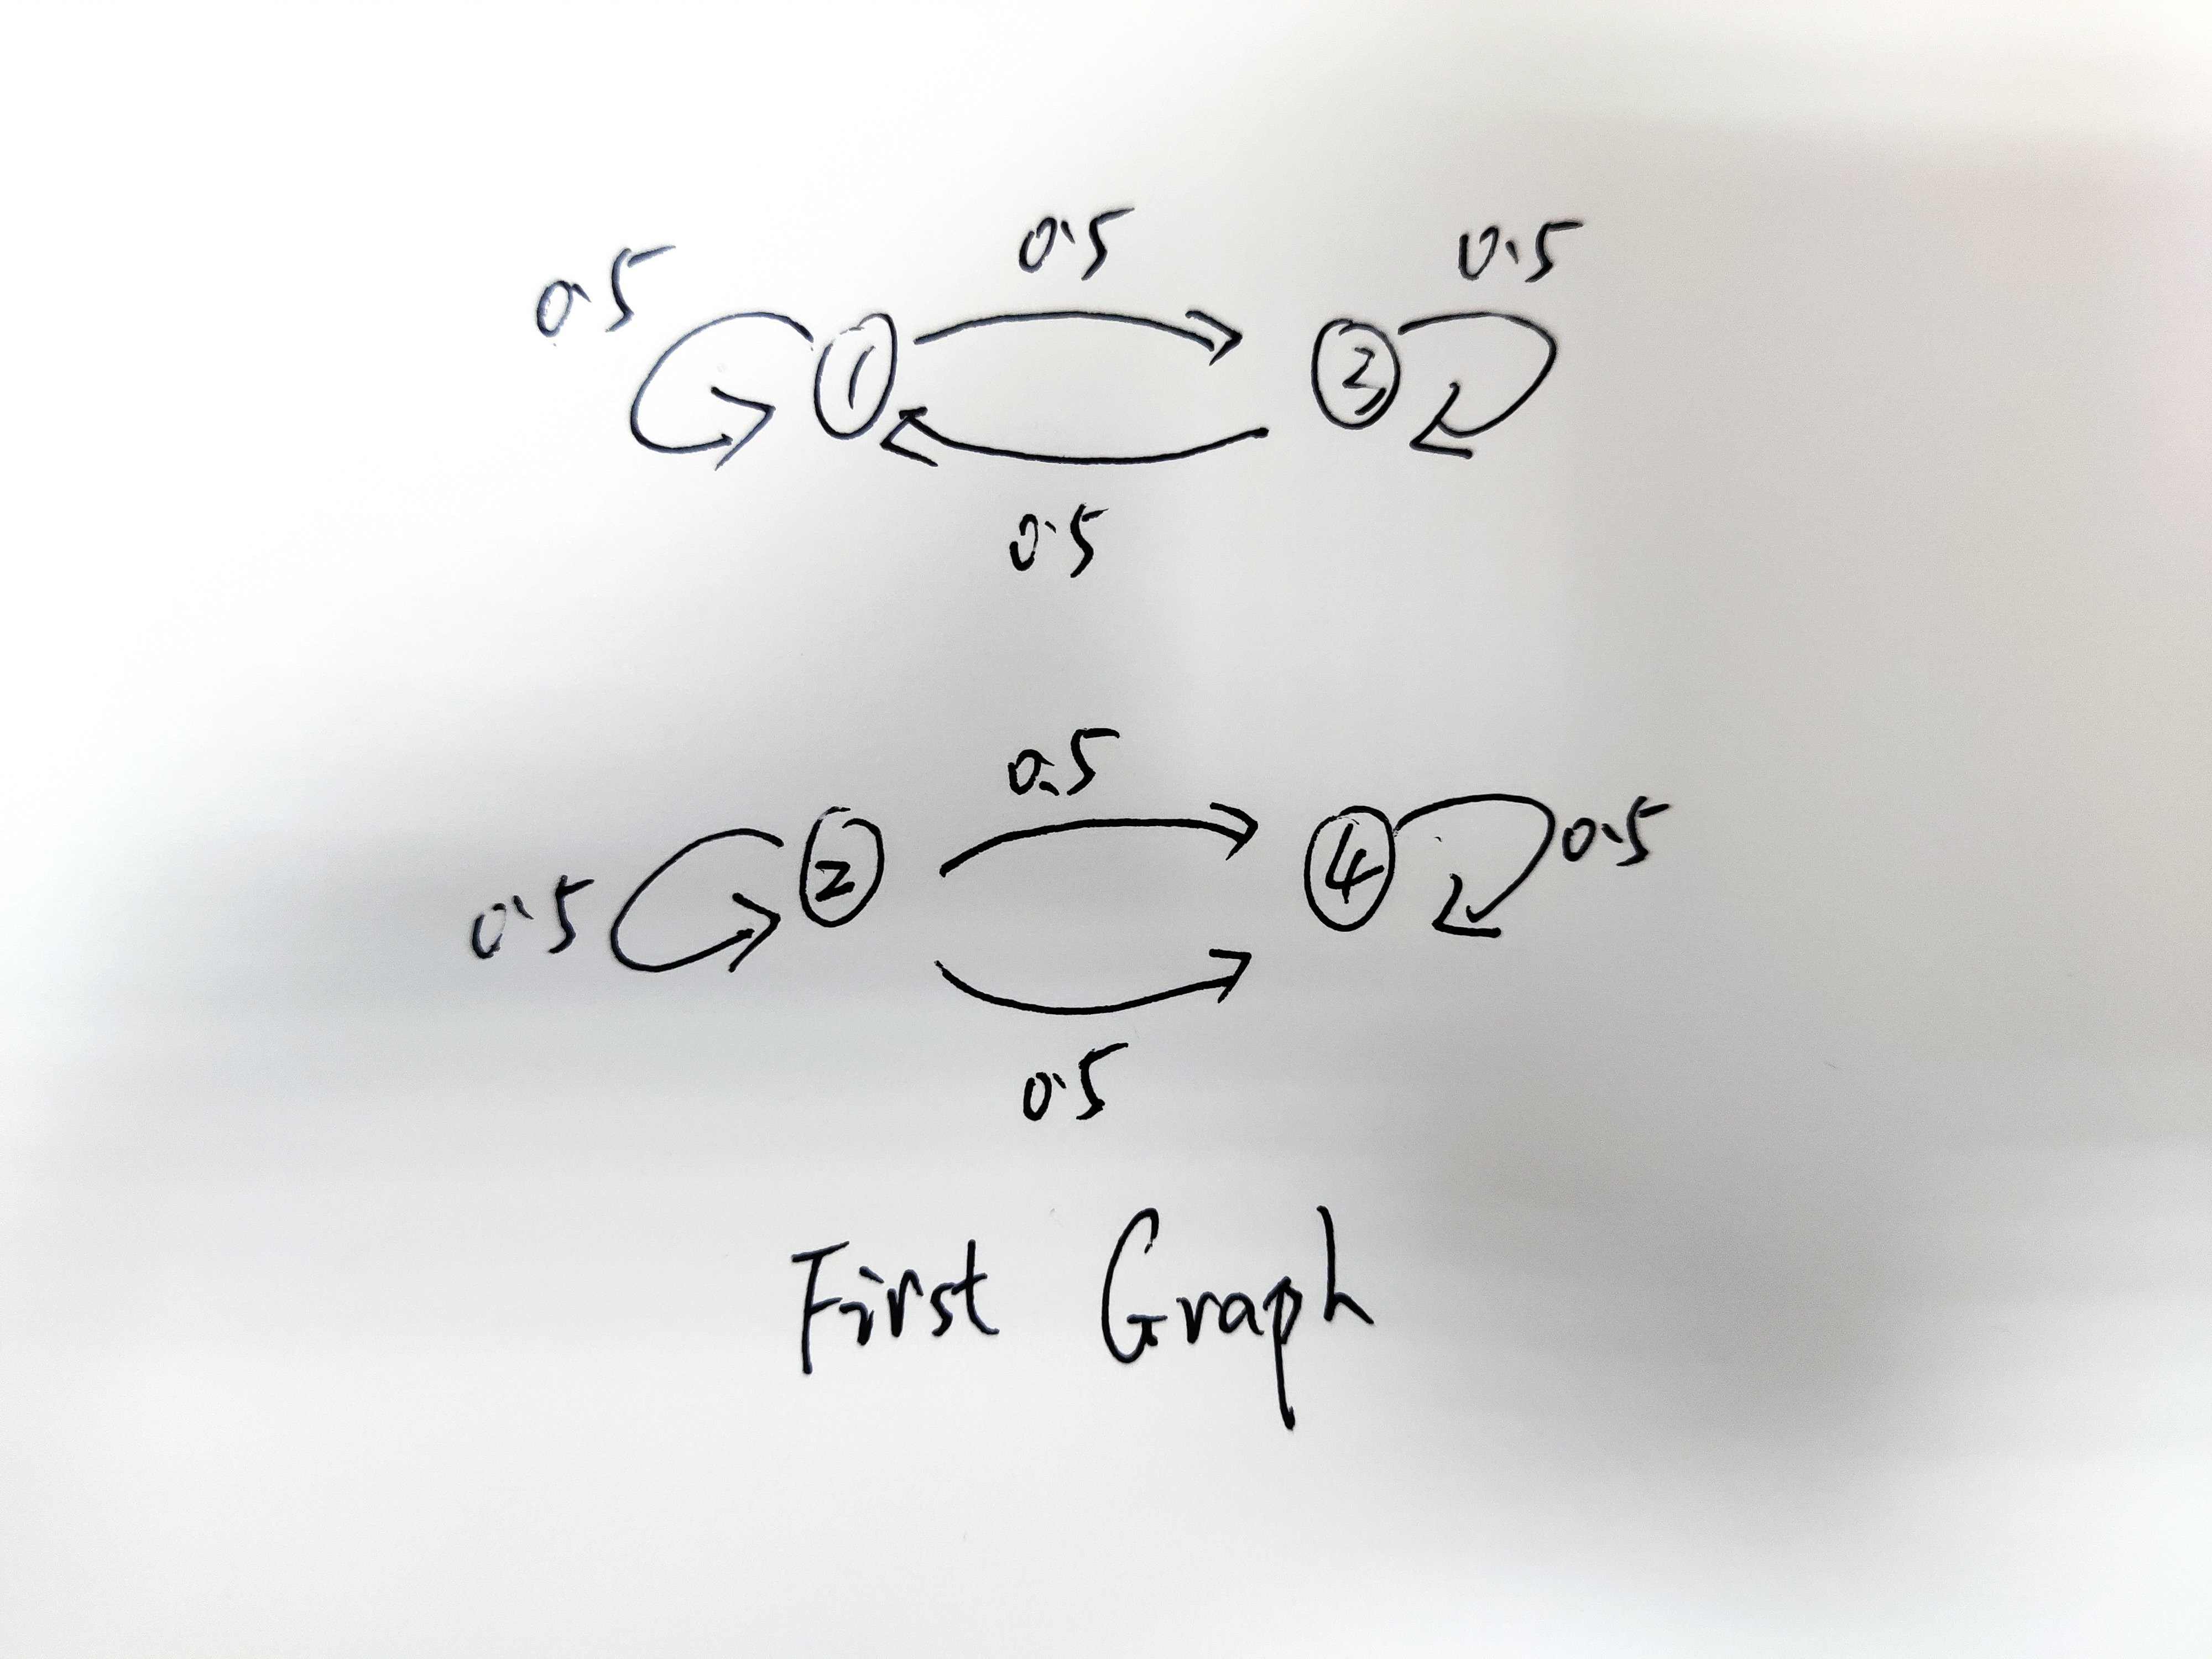
\includegraphics[width=3.0in]{first.jpg}
            \end{figure}
            \begin{figure}[h]
                \centering
                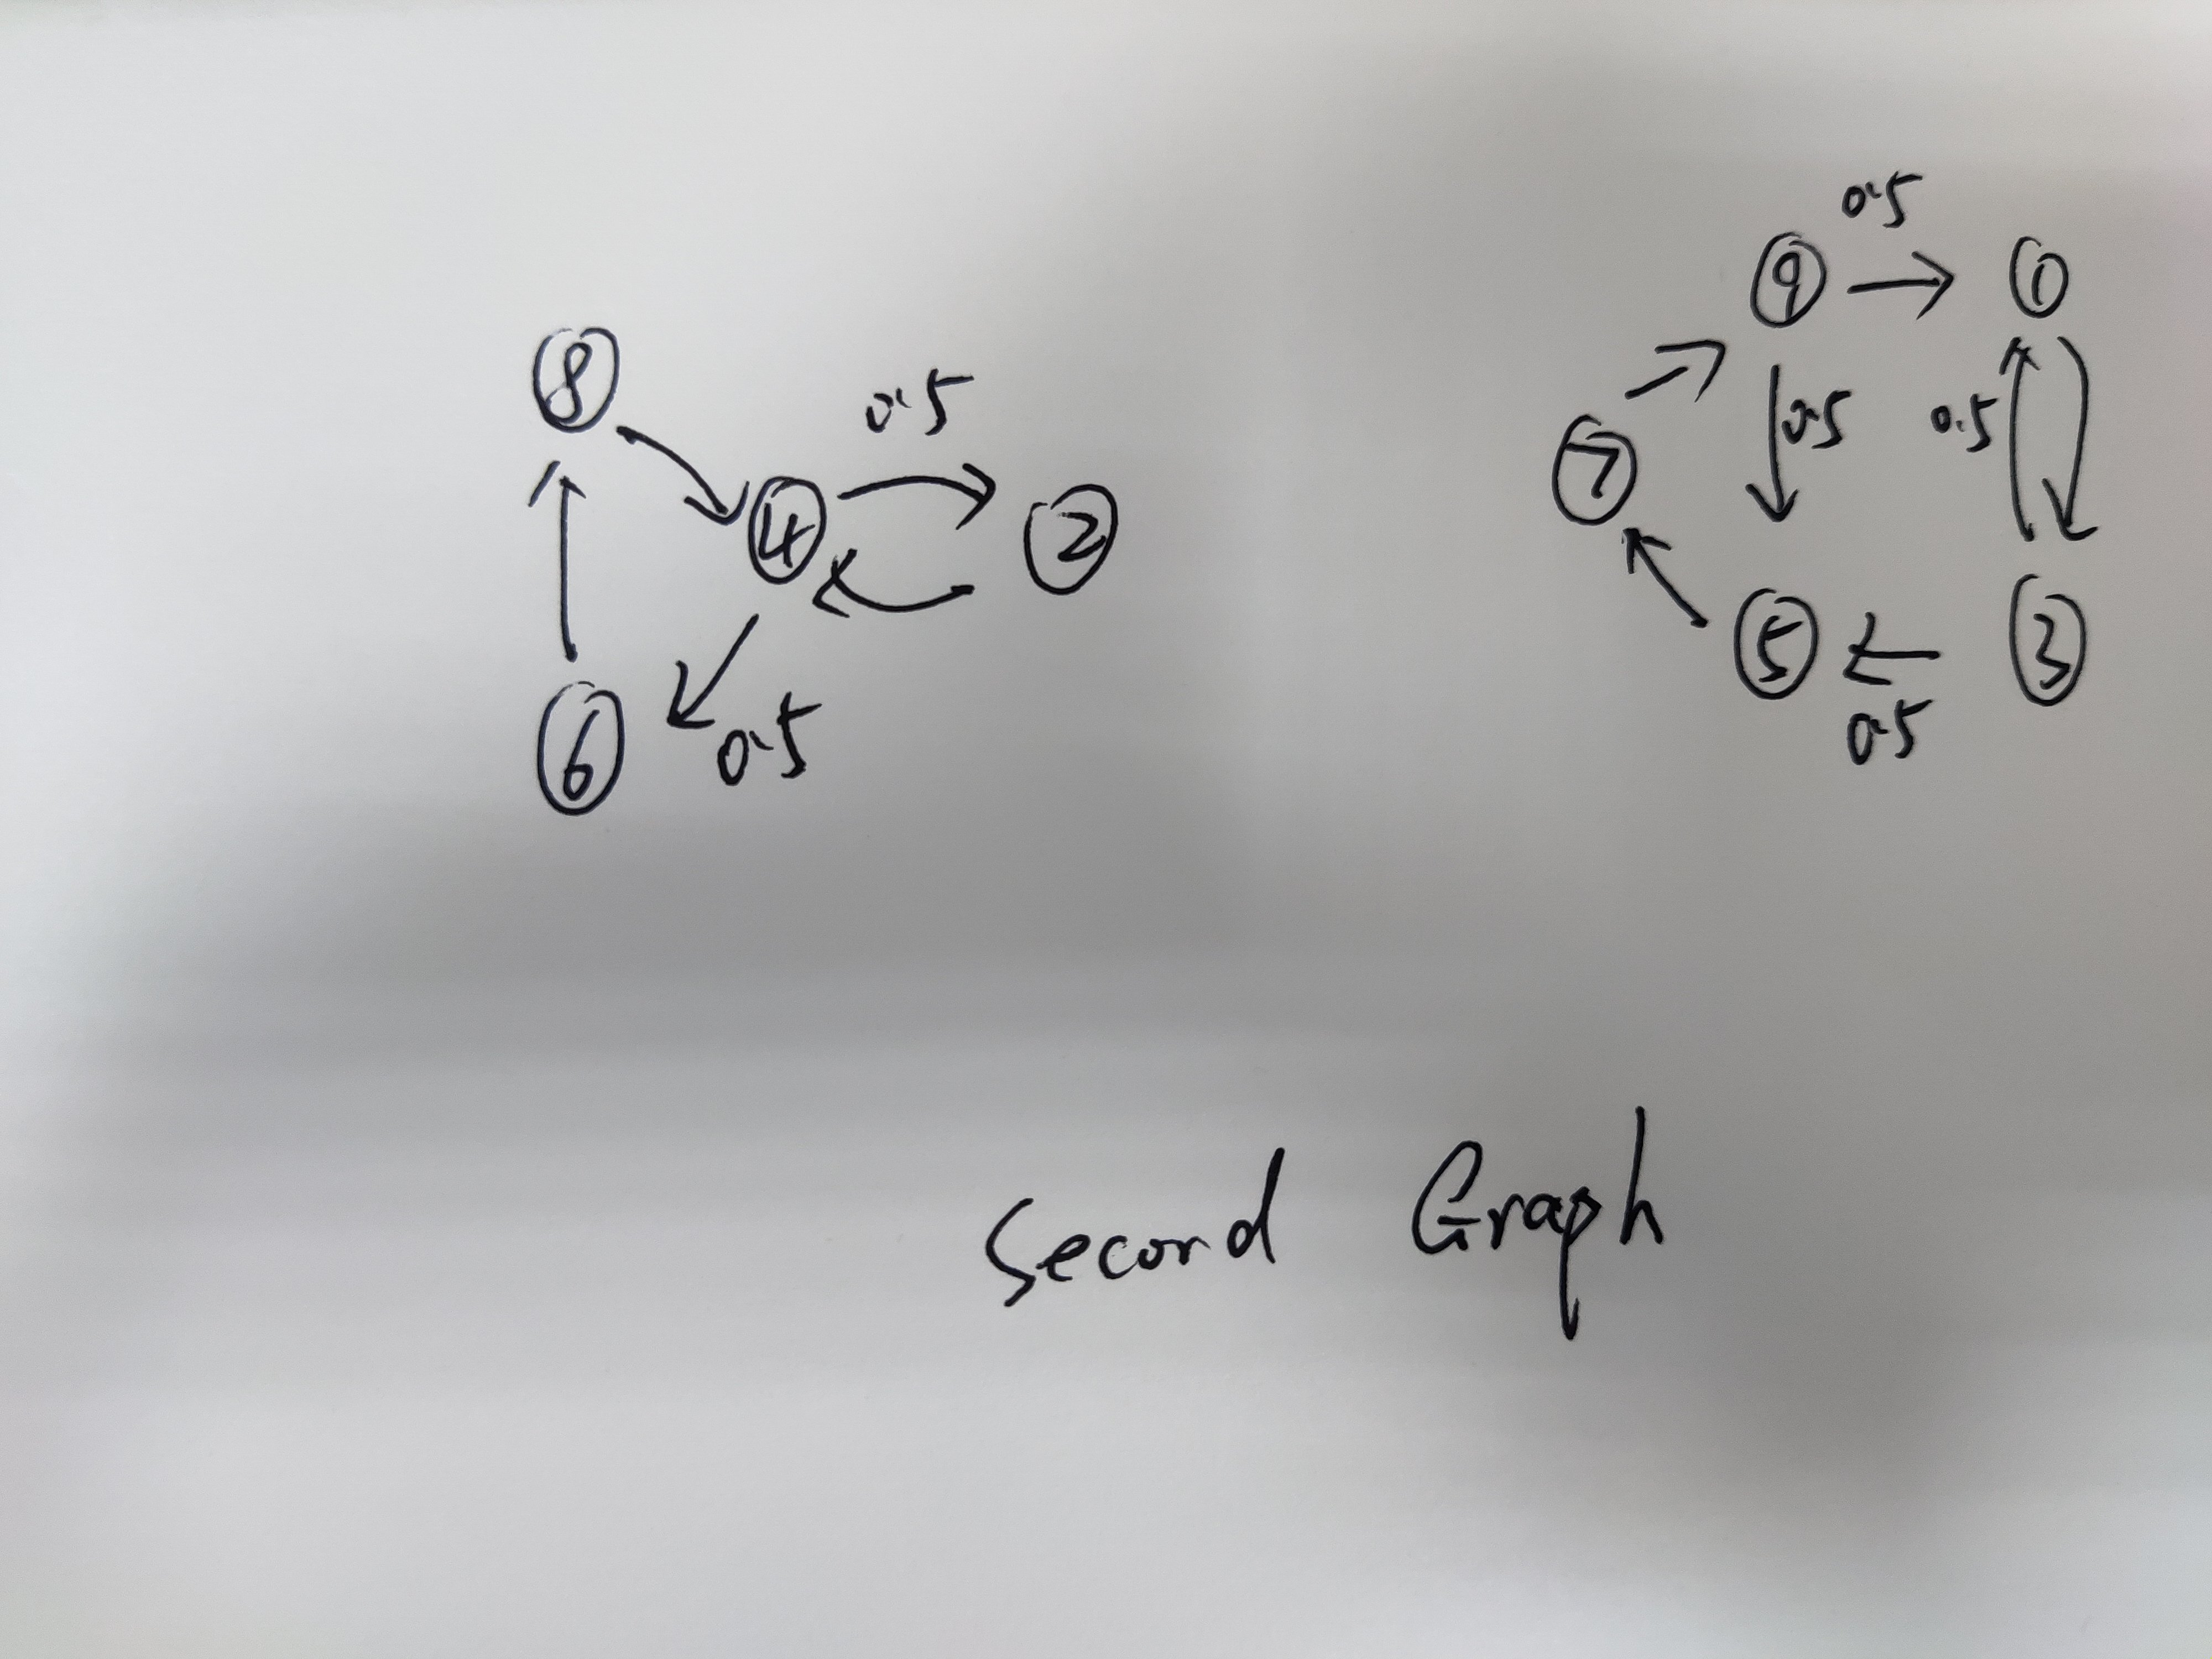
\includegraphics[width=3.0in]{second.jpg}
            \end{figure}
            We can see that there exists two recurrent class of $[P^2]$ for both two graphs.
        \item The limit for each of the chains can be block diagonal, where one block represents the even numbers and the other one represents the odd numbers. Each chain of the block is aperiodic and has a single class, and thus the components of steady-state vector of each sub chain  are all the same, such as $\frac{1}{M}$ where M is the amount of states in each block.
    \end{enumerate}

    \section{Exercise 4.12}
    \begin{enumerate}[(a)]
        \item Let $\lambda_k$ be an eigenvalue of a stochastic matrix $[P]$ and let $\bm{\pi}^{(k)}$ be a left eigenvector for $\lambda_k$. Show that for each component $\pi_j^{(k)}$ of $\bm{\pi}^{(k)}$ and each $n$ that
        \begin{equation*}
            \lambda^n_k\pi_j^{(k)}=\sum_i\pi_i^{(k)}P^n_{ij}
        \end{equation*} 
        \item By taking magnitudes of each side and looking at the appropriate $j$, show that
        \begin{equation*}
            |\lambda_k|^n\leq\text{M}
        \end{equation*}
        \item Show that $|\lambda_k|\leq 1$.
    \end{enumerate}
    \textbf{Solutions:}
    \begin{enumerate}[(a)]
        \item Firstly, we can obtain that
            \begin{equation*}
                \bm{\pi}^{(k)}[P]=\lambda_k\bm{\pi}^{(k)}
            \end{equation*}
            Then,
            \begin{equation*}
                \bm{\pi}^{(k)}[P^2]=\bm{\pi}^{(k)}[P][P]=\lambda_k\bm{\pi}^{(k)}[P]=\lambda_k^2\bm{\pi}^{(k)}
            \end{equation*}
            By applying the method above repeatedly, we can obtain that:
            \begin{equation*}
                \bm{\pi}^{(k)}[P^n]=\lambda^n_k\bm{\pi}^{(k)}
            \end{equation*}

            which is the equivalent form of $\lambda^n_k\pi_j^{(k)}=\sum_i\pi_i^{(k)}P^n_{ij}$.
        \item Suppose that
            \begin{equation*}
                |\pi_j^{(k)}|\geq|\pi_i^{(k)}|\quad\text{for }i=1,\dots,M 
            \end{equation*}

            Then
            \begin{equation*}
                |\lambda_k|^n|\pi_j^{(k)}|=|\sum_i\pi_i^{(k)}P_{ij}^n|\leq\sum_i|\pi^{(k)}_i|P_{ij}^n\leq M|\pi_j^{(k)}|
            \end{equation*}

            Thus, $|\lambda_k|^n\leq M$.

        \item Subsitute $n=1$ to (b) can obtain the result directly.
    \end{enumerate}

    \section{Exercise 4.14}
    Answer the following questions for the following stochastic matrix $[P]$:
    \begin{equation*}
        [P]=\begin{bmatrix}
            1/2 & 1/2 & 0\\
            0 & 1/2 & 1/2\\
            0 & 0 & 1
            \end{bmatrix}
    \end{equation*}

    \begin{enumerate}[(a)]
        \item Find $[P^n]$ in closed form for arbitrary $n>1$.
        \item Find all distinct eigenvalues and the multiplicity of each eigenvalue for $[P]$.
        \item Find a right eigenvector for each distinct eigenvalue, and show that the eigenvalue of multiplicity 2 does not have two linearly independent eigenvectors.
        \item Use (c) to show that there is no diagonal matrix $[\Lambda]$ and no invertible matrix $[U]$ for which $[P][U]=[U][\Lambda]$.
        \item Rederive the result of (d) using the result of (a) rather than (c).
    \end{enumerate}

    \textbf{Solutions:}
    \begin{enumerate}[(a)]
        \item 
        \begin{equation*}
            \begin{aligned}
                &P^n_{11} = (P_{11})^n=2^{-n}\\
                &P^n_{12} = P_{12}\sum_{k=0}^{n-1}P^k_{11}P_{22}^{n-k+1} =n2^{-n}\\
                &P^n_{13} = 1 - P_{11}^n-P^n_{12} = 1-(n+1)2^{-n}\\
                &P^n_{22} = (P_22)^n=2^{-n}\\
                &P^n_{23} = 1- P^n_{22} = 1-2^{-n}\\
                &P^n_{33} = (P_{33}^n)=1
            \end{aligned}
        \end{equation*}

        Thus,
        \begin{equation*}
            [P^n]=\begin{bmatrix}
                2^{-n} & n2^{-n} & 1-(n+1)2^{-n}\\
                0 & 2^{-n} & 1-2^{-n}\\
                0 & 0 & 1\\
            \end{bmatrix}
        \end{equation*}
        \item 
        \begin{equation*}
            \det[P-\lambda I]=(\frac{1}{2}-\lambda)^2(1-\lambda) = 0
        \end{equation*}
        Thus, $\lambda=1$ is an eigenvalue of multiplicity 1 and $\lambda=\frac{1}{2}$ is an eigenvalue of multiplicity 2.

        \item
        For $\lambda=1$, the right eigenvector is $\vec{\nu}=(1, 1, 1)$

        For $\lambda=\frac{1}{2}$, solve the following equation $[P-\lambda I]\vec{\nu}=\vec{0}$,
        \begin{equation*}
            \begin{bmatrix}
                0 & \frac{1}{2} & 0\\
                0 & 0 & \frac{1}{2}\\
                0 & 0 & \frac{1}{2}
            \end{bmatrix}\vec{\nu}=\vec{0}
        \end{equation*}
        And thus, $\vec{\nu}=(1,0,0)^\text{T}$ is unique within a scale factor. Therefore,  the eigenvalue of multiplicity 2 does not have two linearly independent eigenvectors.
        \item Letting $\bm{\nu}^1,\bm{\nu}^2,\bm{\nu}^3$ be the columns of $[U]$, and thus $[P][U]=[U][\Lambda]$ can be written as  $[P]\bm{\nu}_i=\lambda_v\bm{\nu}_i$ for $i=1,2,3$. If $[U]$ is invertible, $\bm{\nu}_1,\bm{\nu}_2,\bm{\nu}_3$ must be linearly independent eigenvectors of $[P]$. But (c) has showed that such three eigenvectors do not exist.
        \item If such $[\Lambda]$ and $[U]$ exist, then $[P^n]=[U][\Lambda^n][U^{-1}]=\sum_{i=1}^3\lambda^n_i\bm{\nu}^i\bm{\pi}^i$ where $\bm{\nu}^i$ is th $i$th column of $[U]$ and $\bm{\pi}^i$ is the $i$th row of $[U^{-1}]$. Since $P^n_{12}=n2^{-n}\neq\sum_{i=1}^3\lambda^n_i\bm{\nu}^1\bm{\pi}^2$, there is a contradiction.
    \end{enumerate} 
\end{document}